\subsubsection{Architektur}

Die Architektur lässt sich grob in zwei Komponenten (Fotoshoot UI/Raspi Controller) einteilen. Das Komponentendiagramm in Abbildung \ref{fig:komponentendiagramm} zeigt eine Übersicht über die Architektur. Beim Fotoshoot UI handelt es sich um ein Java Programm welches auf einem beliebigen Computer mit Java ausführen lässt. Es dient zur Steuerung der Maschine. Der Raspi Controller wird auf dem Raspberry Pi ausgeführt und verarbeitet die Befehle vom Fotoshoot UI.

\begin{figure}[h!]
	\centering
	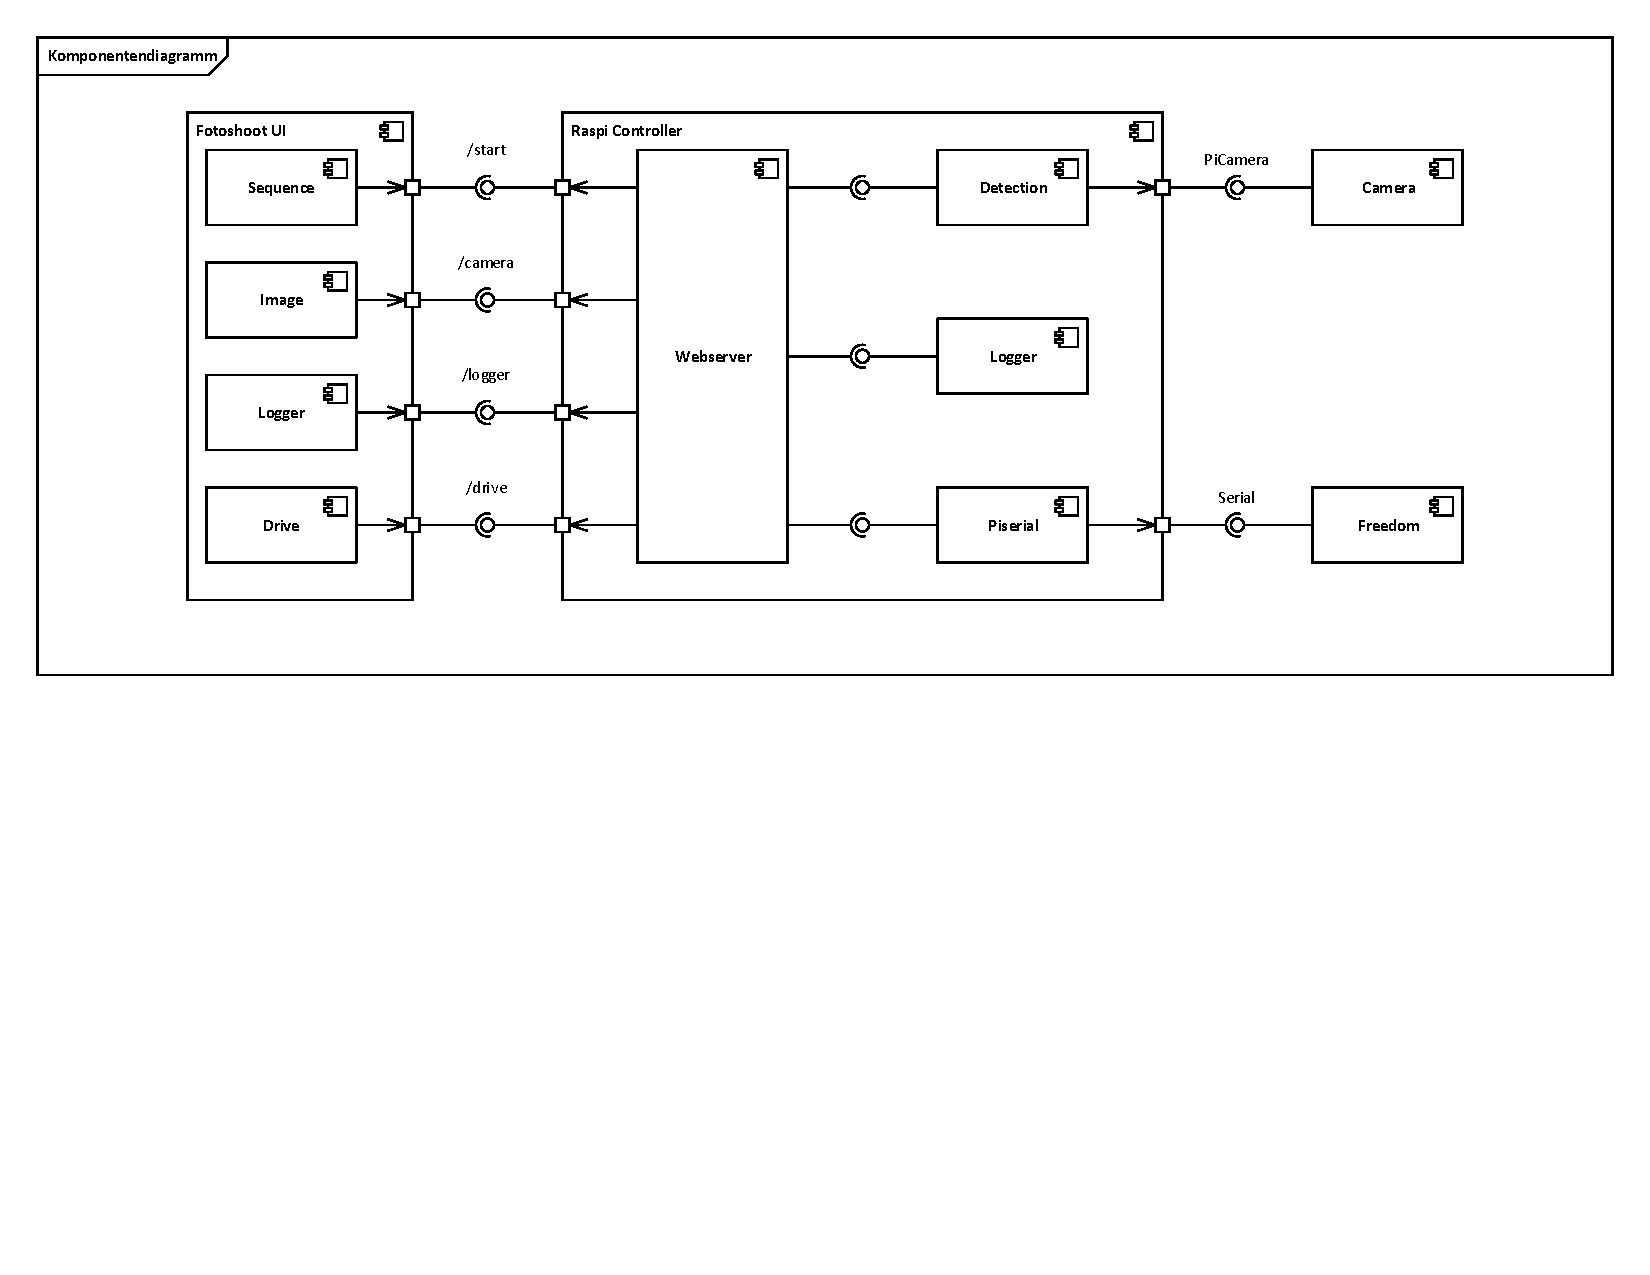
\includegraphics[width=\linewidth]{../../fig/komponentendiagramm}
	\caption{Komponentendiagramm}
	\label{fig:komponentendiagramm}
\end{figure}

Auf dem Raspi Controller wird ein Webserver ausgeführt, welcher über eine REST-Schnittstelle Befehle entgegen nimmt. Diese REST-Schnittstelle ermöglicht eine unabhängige Entwicklung der beiden Komponenten. Die Anfragen an der Webserver werden an weitere Komponenten innerhalb des Raspi Controllers weitergeleitet. Die Komponenten vom Raspi Controller wurde gemäss den Hauptfunktionen der Maschine aufgeteilt. Die Detection-Komponente erzeugt mit Hilfe der Camera-Komponente ein Bild und erkennt darauf den Korb. Die PiSerial-Komponente ist für die Ansteuerung der seriellen Schnittstelle und damit für die Kommunikation mit dem Freedom-Board zuständig. Mit dem Freedom-Board werden sämtliche Motoren angesteuert. Zusätzliche wurde noch eine Logger-Komponente entwickelt, welche für das Logging zuständig ist. Die Log-Einträge können über den Webserver abgerufen und auf dem UI dargestellt werden.

Die Komponenten vom Fotoshoot UI wurden gemäss den UI-Ansichten aufgeteilt. So gibt es beispielsweise eine UI-Ansicht für die Steuerung der Motoren. Alle Funktionen welche für diese Aufgabe benötigt werden, sind demzufolge in der Drive-Komponente zu finden.

In den nachfolgenden Abschnitten wird jeweils auf die Komponenten des Komponentendiagramms \ref{fig:komponentendiagramm} eingegangen.